\documentclass[12pt,a4paper]{article}
\usepackage[T1]{fontenc}
%\usepackage[latin1]{inputenc}
%\usepackage{amssymb,amsmath,a4wide}
\usepackage[utf8]{inputenc}
\usepackage{amssymb,amsmath}
\usepackage{nicefrac}
\usepackage[pdftex]{graphicx}
\usepackage{ctable}
\usepackage{amsmath}
%\usepackage{threeparttable} %na
%\usepackage{tabu} %na
\usepackage{tabularx}
\usepackage{subfig}
\usepackage{rotating}
\usepackage{longtable}
%\usepackage[table]{xcolor} % clash with floatrow
\usepackage{xcolor} 
\usepackage{floatrow}
\usepackage{threeparttable}
%\usepackage[multiple]{footmisc} %na
\usepackage{bm}
\usepackage{fancybox}
%\usepackage{harvard}
\usepackage{geometry}         % Definir les marges
\geometry{verbose,a4paper,tmargin=1in,bmargin=1in,lmargin=1in,rmargin=1in}
\usepackage{setspace}
%\usepackage{ccaption}
\usepackage[colorlinks=true,citecolor=black, urlcolor=black, linkcolor=black]{hyperref}
\usepackage{url}
\newcommand{\email}[1]{\href{mailto:#1}{\nolinkurl{#1}}}
\usepackage[french, english]{babel}  % Placez ici une liste de langues, la derniere etant la langue principale
\usepackage{lscape}
\usepackage{afterpage}
\usepackage{supertabular}    %na            %  mettre pour les grands tableaux en formant paysage. marche avec \begin{landscape}
% style de la biblio : necessaire pour utiliser BibTex, necessite le deuxieme fichier exemple.bib
\usepackage{caption}
%\usepackage[longnamesfirst]{natbib}
\usepackage{natbib}
\bibliographystyle{elsarticle-harv}
\newcommand{\tqdl}{\textquotedblleft}
\newcommand{\tqdr}{\textquotedblright}
\DeclareUnicodeCharacter{FB01}{fi}
\DeclareUnicodeCharacter{FB00}{ff}
%\linespread{1.2}
\usepackage[title]{appendix}
\usepackage{setspace}
\doublespacing



% !TeX spellcheck = en_US


\begin{document}
\title{Global value chains and the transmission of exchange rate shocks to consumer prices: Online Appendix	\thanks{ All programs and are available at \url{https://github.com/gdaudin/OFCE_CommerceVA}. Data and results files are available upon request.}\\
\vspace{1cm}
}
\vspace{1cm}
\date{\today}
\author{
	Hadrien Camatte\thanks{Banque de France. E-mail: \email{hadrien.camatte@banque-france.fr}}
	\and
	Guillaume Daudin\thanks{Université Paris-Dauphine, PSL University, CNRS, 8007, IRD, 260, LEDa, DIAL, 75016, Paris, France. Sciences Po, OFCE, 75007, Paris. Corresponding author. E-mail: \email{guillaume.daudin@dauphine.psl.eu}}
	\and
	Violaine Faubert\thanks{Banque de France, ECB. E-mail: \email{violaine.faubert@ecb.europa.eu}}
	\and
	Antoine Lalliard\thanks{Banque de France. E-mail: \email{antoine.lalliard@banque-france.fr}}
	\and
	Christine Rifflart\thanks{Sciences Po, OFCE. E-mail: \email{christine.rifflart@sciencespo.fr}}
}
%\vspace*{\fill}
\maketitle

\section*{Online Appendix A: WIOD Sectors}
\begin{table}[H]
 \centering
 \caption{\footnotesize{\textbf{WIOD sectors}}}
 \footnotesize
 \begin{tabular}{ll}
  \hline \\
\textbf{A01} &{Crop and animal production, hunting and related service activities}\\
\textbf{A02} &{Forestry and logging}\\
\textbf{A03} &{Fishing and aquaculture}\\
\textbf{B} &{Mining and quarrying}\\
\textbf{C10-C12} &{Manufacture of food products, beverages and tobacco products}\\
\textbf{C13-C15} &{Manufacture of textiles, wearing apparel and leather products}\\
\textbf{C16} &{Manufacture of wood and of products of wood and cork, except furniture; articles of straw and plaiting materials}\\
\textbf{C17} &{Manufacture of paper and paper products}\\
\textbf{C18} &{Printing and reproduction of recorded media}\\
\textbf{C19} &{Manufacture of coke and refined petroleum products}\\
\textbf{C20} &{Manufacture of chemicals and chemical products}\\
\textbf{C21} &{Manufacture of basic pharmaceutical products and pharmaceutical preparations}\\
\textbf{C22} &{Manufacture of rubber and plastic products}\\
\textbf{C23} &{Manufacture of other non-metallic mineral products}\\
\textbf{C24} &{Manufacture of basic metals}\\
\textbf{C25} &{Manufacture of fabricated metal products, except machinery and equipment}\\
\textbf{C26} &{Manufacture of computer, electronic and optical products}\\
\textbf{C27} &{Manufacture of electrical equipment}\\
\textbf{C28} &{Manufacture of machinery and equipment n.e.c.}\\
\textbf{C29} &{Manufacture of motor vehicles, trailers and semi-trailers}\\
\textbf{C30} &{Manufacture of other transport equipment}\\
\textbf{C31-C32} &{Manufacture of furniture; other manufacturing}\\
\textbf{C33} &{Repair and installation of machinery and equipment}\\
\textbf{D35} &{Electricity, gas, steam and air conditioning supply}\\
\textbf{E36} &{Water collection, treatment and supply}\\
\textbf{E37-E39} &{Sewerage and other waste management services}\\
\textbf{F} &{Construction}\\
\textbf{G45} &{Wholesale and retail trade and repair of motor vehicles and motorcycles}\\
\textbf{G46} &{Wholesale trade, except of motor vehicles and motorcycles}\\
\textbf{G47} &{Retail trade, except of motor vehicles and motorcycles}\\
\textbf{H49} &{Land transport and transport via pipelines}\\
\textbf{H50} &{Water transport}\\
\textbf{H51} &{Air transport}\\
\textbf{H52} &{Warehousing and support activities for transportation}\\
\textbf{H53} &{Postal and courier activities}\\
\textbf{I} &{Accommodation and food service activities}\\
\textbf{J58} &{Publishing activities}\\
\textbf{J59-J60} &{Motion picture, video and television programme production; programming and broadcasting activities}\\
\textbf{J61} &{Telecommunications}\\
\textbf{J62-J63} &{Computer programming, consultancy; information service activities}\\
\textbf{K64} &{Financial service activities, except insurance and pension funding}\\
\textbf{K65} &{Insurance, reinsurance and pension funding, except compulsory social security}\\
\textbf{K66} &{Activities auxiliary to financial services and insurance activities}\\
\textbf{L68} &{Real estate activities}\\
\textbf{M69-M70} &{Legal and accounting activities}\\
\textbf{M71} &{Architectural and engineering activities; technical testing and analysis}\\
\textbf{M72} &{Scientific research and development}\\
\textbf{M73} &{Advertising and market research}\\
\textbf{M74-M75} &{Other professional, scientific and technical activities; veterinary activities}\\
\textbf{N} &{Administrative and support service activities}\\
\textbf{O84} &{Public administration and defence; compulsory social security}\\
\textbf{P85} &{Education}\\
\textbf{Q} &{Human health and social work activities}\\
\textbf{R-S} &{Other service activities}\\
\textbf{T} &{Activities of households as employers; producing activities of households for own use}\\
\textbf{U} &{Activities of extraterritorial organizations and bodies}\\
  	\end{tabular}
\label{tab:wiodindustries}
\end{table}

\newpage
\section*{Online appendix B: Comparison of $S$ and $S^i$ in the two-country, one-sector case}
In this appendix, we use the two-country and one-good case to illustrate the difference between a price shock  and an exchange rate shock.
\subsection*{Effect of a price shock based of VA contents}
Using the notations of the paper, we have in the two-country and one good case:
\begin{gather*}
\cal {A} = \left(\begin{matrix}a_{1,1}&a_{1,2}\\a_{2,1}&a_{2,2}\end{matrix}\right)
\\
I-\cal {A}=\left(\begin{matrix}1-a_{1,1}&-a_{1,2}\\-a_{2,1}&1-a_{2,2}\end{matrix}\right)
\\
\left(I-\cal {A}\right)^{-1}=\frac{1}{\left(1-a_{1,1}\right)\left(1-a_{2,2}\right)-a_{2,1}a_{1,2}}\left(\begin{matrix}1-a_{2,2}&a_{1,2}\\a_{2,1}&1-a_{1,1}\end{matrix}\right) =z.\left(\begin{matrix}1-a_{2,2}&a_{1,2}\\a_{2,1}&1-a_{1,1}\end{matrix}\right) \\ 
=\left(\begin{matrix}u&v\\w&x\end{matrix}\right)
\\
\text{Country 1 demand shares}=d=\left(\begin{matrix}1-f\\f\end{matrix}\right) \\
\left(I-\cal {A}\right)^{-1}d=\left(\begin{matrix}u-uf+vf\\w-wf+xf\end{matrix}\right)
\end{gather*}

When a shock $c$ occurs on the prices of country 2 (the currency does not matter here), we have the following initial shock vector : $C=\left(0,c\right)$.
In the first instance, this has an impact on prices $C\cal {A}$, and then $C{\cal{A}}^{2}$, etc.
Hence the total effect of the shock $S$ is: 


\begin{equation*}
S=C+C{\cal{A}}+C{\cal{A}}^{2}...=C\left(I-{\cal{A}}\right)^{-1}=\left(\begin{matrix}cw  &   cx\end{matrix}\right)
\end{equation*}

To measure the effect on the French household consumption expenditure deflator, we compute a weighted sum of these effects.

\begin{equation}
\bar{s}=c.\left[\left(1-f\right)w+xf\right]=c.\frac{\left(1-f\right)a_{2,1}+f\left(1-a_{1,1}\right)}{\left(1-a_{1,1}\right)\left(1-a_{2,2}\right)-a_{2,1}a_{1,2}}
\end{equation}

If each nation's production only uses national inputs, we have:
\begin{equation*}
\bar{s}=c.\frac{f}{1-a_{2,2}}
\end{equation*}

\subsection*{Exchange rate shock}

Using the notations in the paper, we have:

\begin{gather*}
C=\left(0,\frac{-c_\$}{1+c_\$}\right)=\left(0,-c\right)
\\
C_\$=\left(c_\$,0\right)
\\
\tilde{C}_\$=\left(0,-c_\$\right)
\\
\hat{C}_\$=\left(\frac{c_\$}{1+c_\$},0\right)=\left(c,0\right)
\\
{\cal B} = \left(\begin{matrix}0&a_{1,2}\\0&0\end{matrix}\right)
\\
\tilde{\cal B} = \left(\begin{matrix}0&0\\a_{2,1}&0\end{matrix}\right)
\end{gather*}

Hence

\begin{gather*}
S =\left(0,c\right)+\left[\left(0,-c.a_{1,2}\right)+\left(c.a_{2,1},0\right)\right]*\left(\begin{matrix}u&v\\w&x\end{matrix}\right)
\\
=\left(0,c\right)+\left(c.a_{2,1},-c.a_{1,2}\right)*\left(\begin{matrix}u&v\\w&x\end{matrix}\right)
\\
=\left(0,c\right)+\left(u.c.a_{2,1}-w.c.a_{1,2},v.c.a_{2,1}-x.c.a_{1,2}\right)
\\
=\left(u.c.a_{2,1}-w.c.a_{1,2},c+v.c.a_{2,1}-x.c.a_{1,2}\right)
\end{gather*}
and
\begin{gather*}
\bar{s}=\left(u.c.a_{2,1}-w.c.a_{1,2},c+v.c.a_{2,1}-x.c.a_{1,2}\right).\left(\begin{matrix}1-f\\f\end{matrix}\right)
\\
\bar{s}=c\left[f\left(1+v.a_{2,1}-x.a_{1,2}\right)+\left(1-f\right)\left(u.a_{2,1}-w.a_{1,2}\right)\right]
\end{gather*}


If each nation's production only uses national inputs, we have a plausible

\begin{gather*}
\bar{s}=c.f
\end{gather*}

This confirms that an exchange rate shock differs from a price shock.

\newpage
\section*{Online Appendix C: Comparision of $\overline{s}_{i}^{i,HC}$ and $E1.HC^{i,imp}+E2.HC^{i,dom}$ in the TIVA rev. 3 and TIVA rev. 4 databases} \label{AppendixFonctionLinéaireTIVA}

Figures \ref{fig:ratiodir_TiVA}, \ref{fig:evolution_b_TiVA} and \ref{fig:evolution_cst_TiVA} for TIVA rev. 3 and Figures \ref{fig:ratiodir_TiVA_REV4}, \ref{fig:evolution_b_TiVA_REV4} and \ref{fig:evolution_cst_TiVA_REV4} for TIVA rev. 4 show that we get a good prediction of the partial equilibrium effects of an exchange rate shock on consumption prices by using simply the share of imported final consumption goods and services and the share of imported intermediate goods in domestic final consumption.




\begin{figure}[H]
	\centering
	\caption{\footnotesize{\textbf{Comparing $\overline{s}_{i}^{i,HC}$ and $E1.HC^{i,imp}+E2.HC^{i,dom}$ (TIVA rev. 3)}}}
	\begin{tabular}{c}
		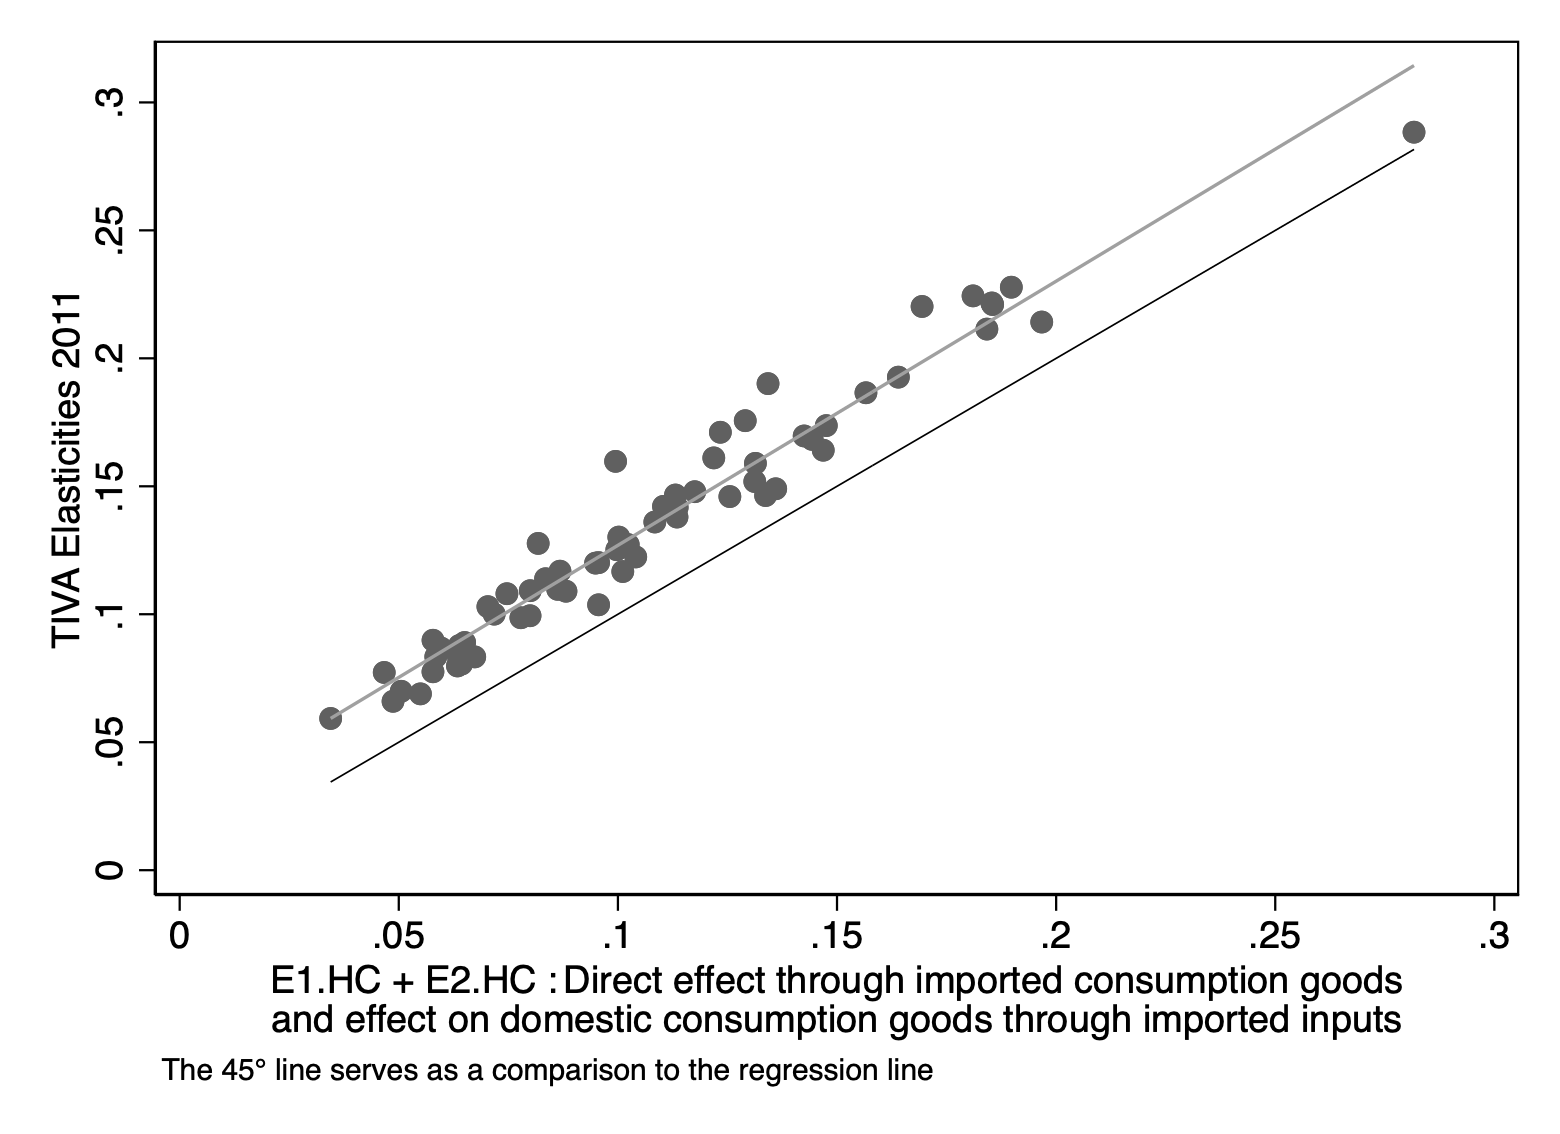
\includegraphics[width=5.0in, height=3.5in]{Comp_s_E1HCE2HC_2011_TIVA_HC.png}\\
	\end{tabular}
	\label{fig:ratiodir_TiVA}
	\floatfoot{Sources: TIVA rev3 and authors’ calculations}.
\end{figure}

\begin{figure}[H]
	\centering
	\caption{\footnotesize{\textbf{Evolution of $\beta$ and $R2$ (TIVA rev. 3)}}}
	\begin{tabular}{c}
		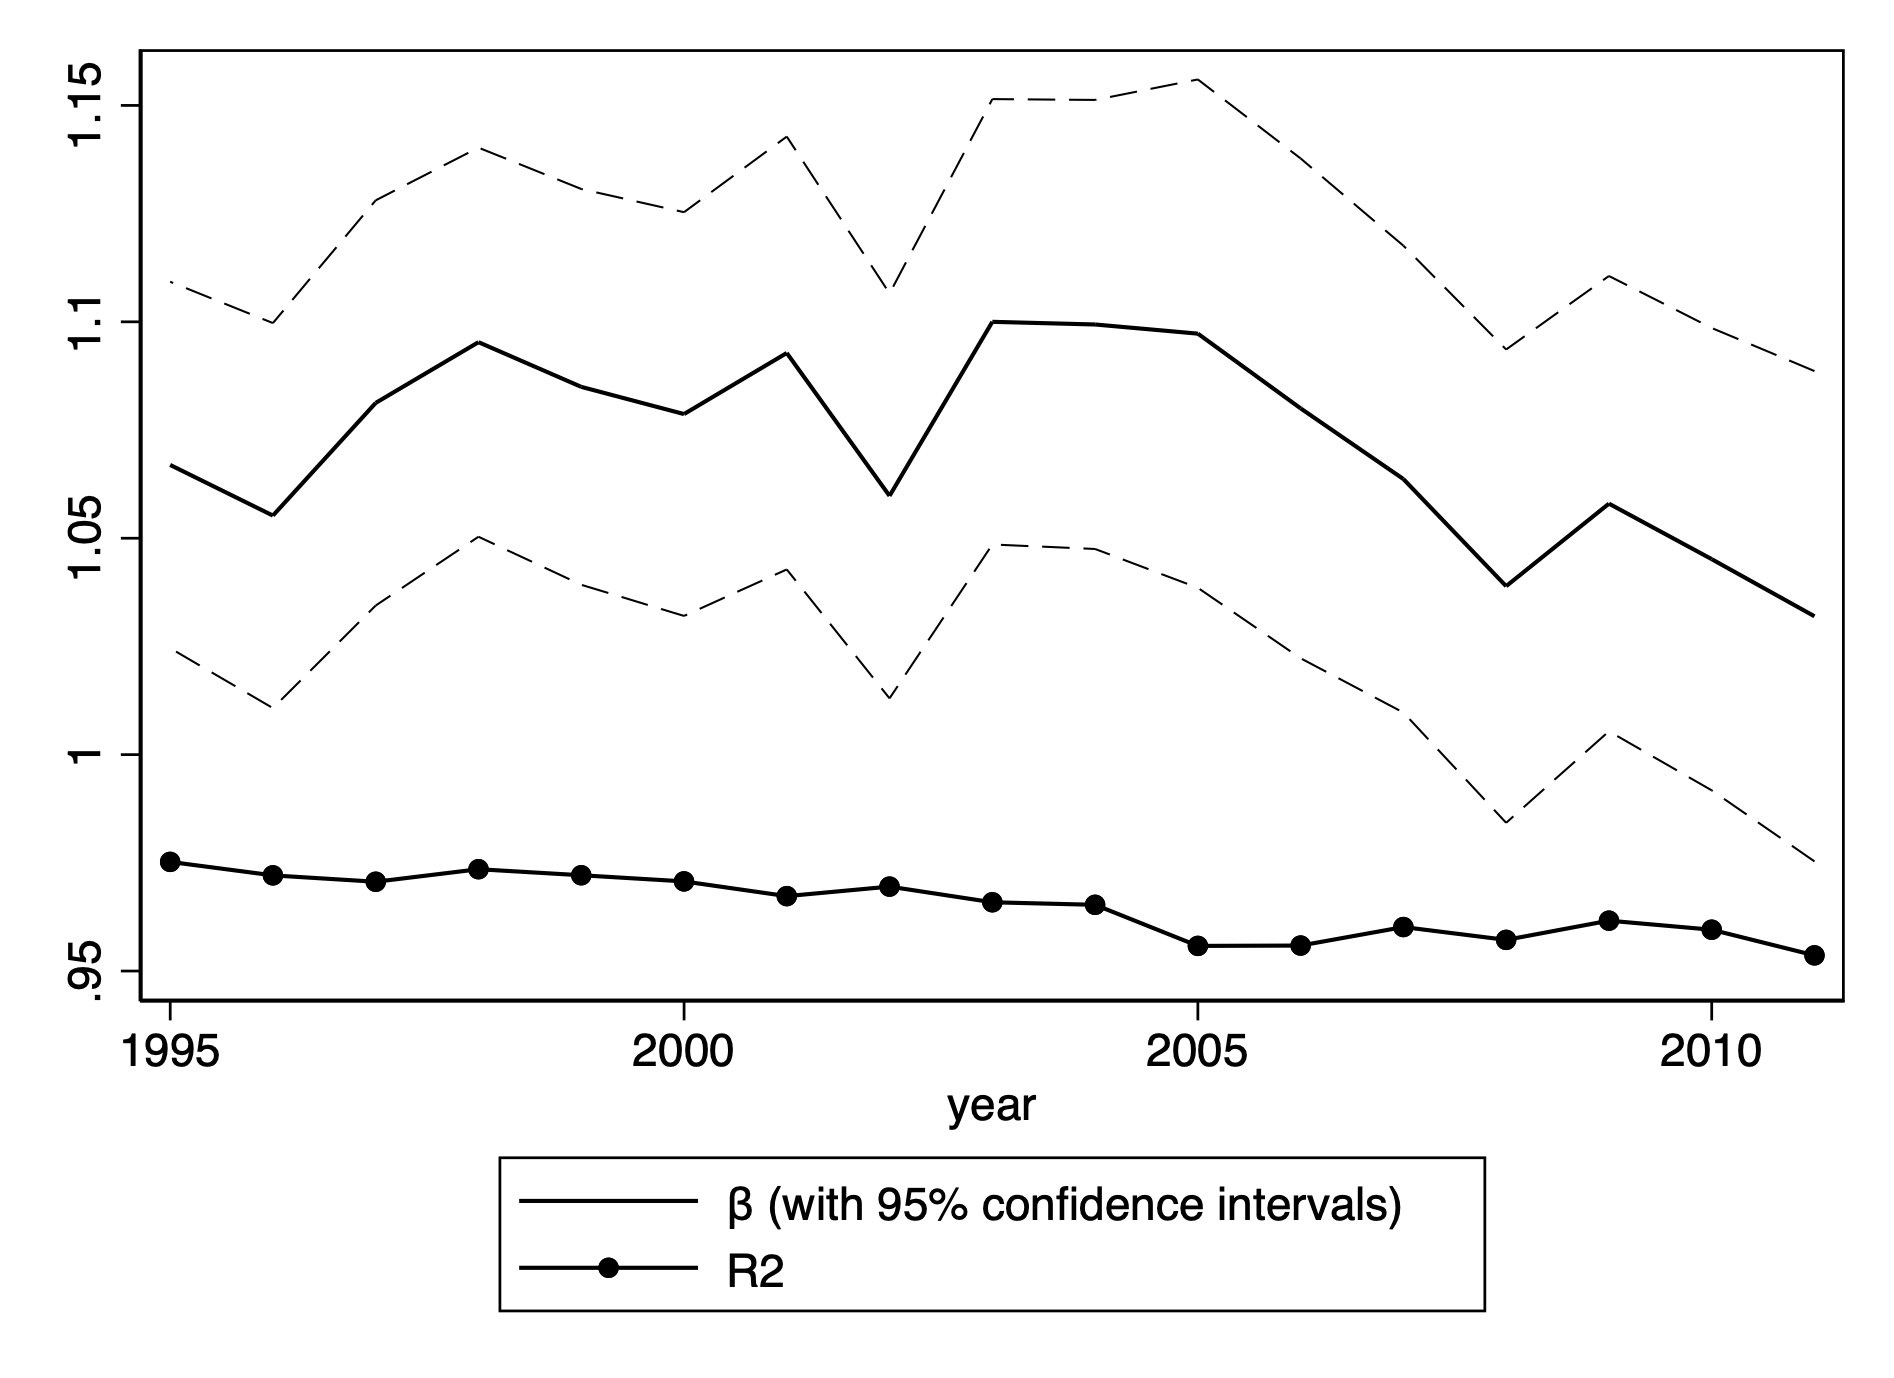
\includegraphics[width=5.0in, height=3.5in]{coef_E_TIVA_HC}\\
	\end{tabular}
	\label{fig:evolution_b_TiVA}
	\floatfoot{Sources: TIVA rev3 and authors’ calculations}.
\end{figure}

\begin{figure}[H]
	\centering
	\caption{\footnotesize{\textbf{Evolution of $\alpha$ (TIVA rev. 3)}}}
	\begin{tabular}{c}
		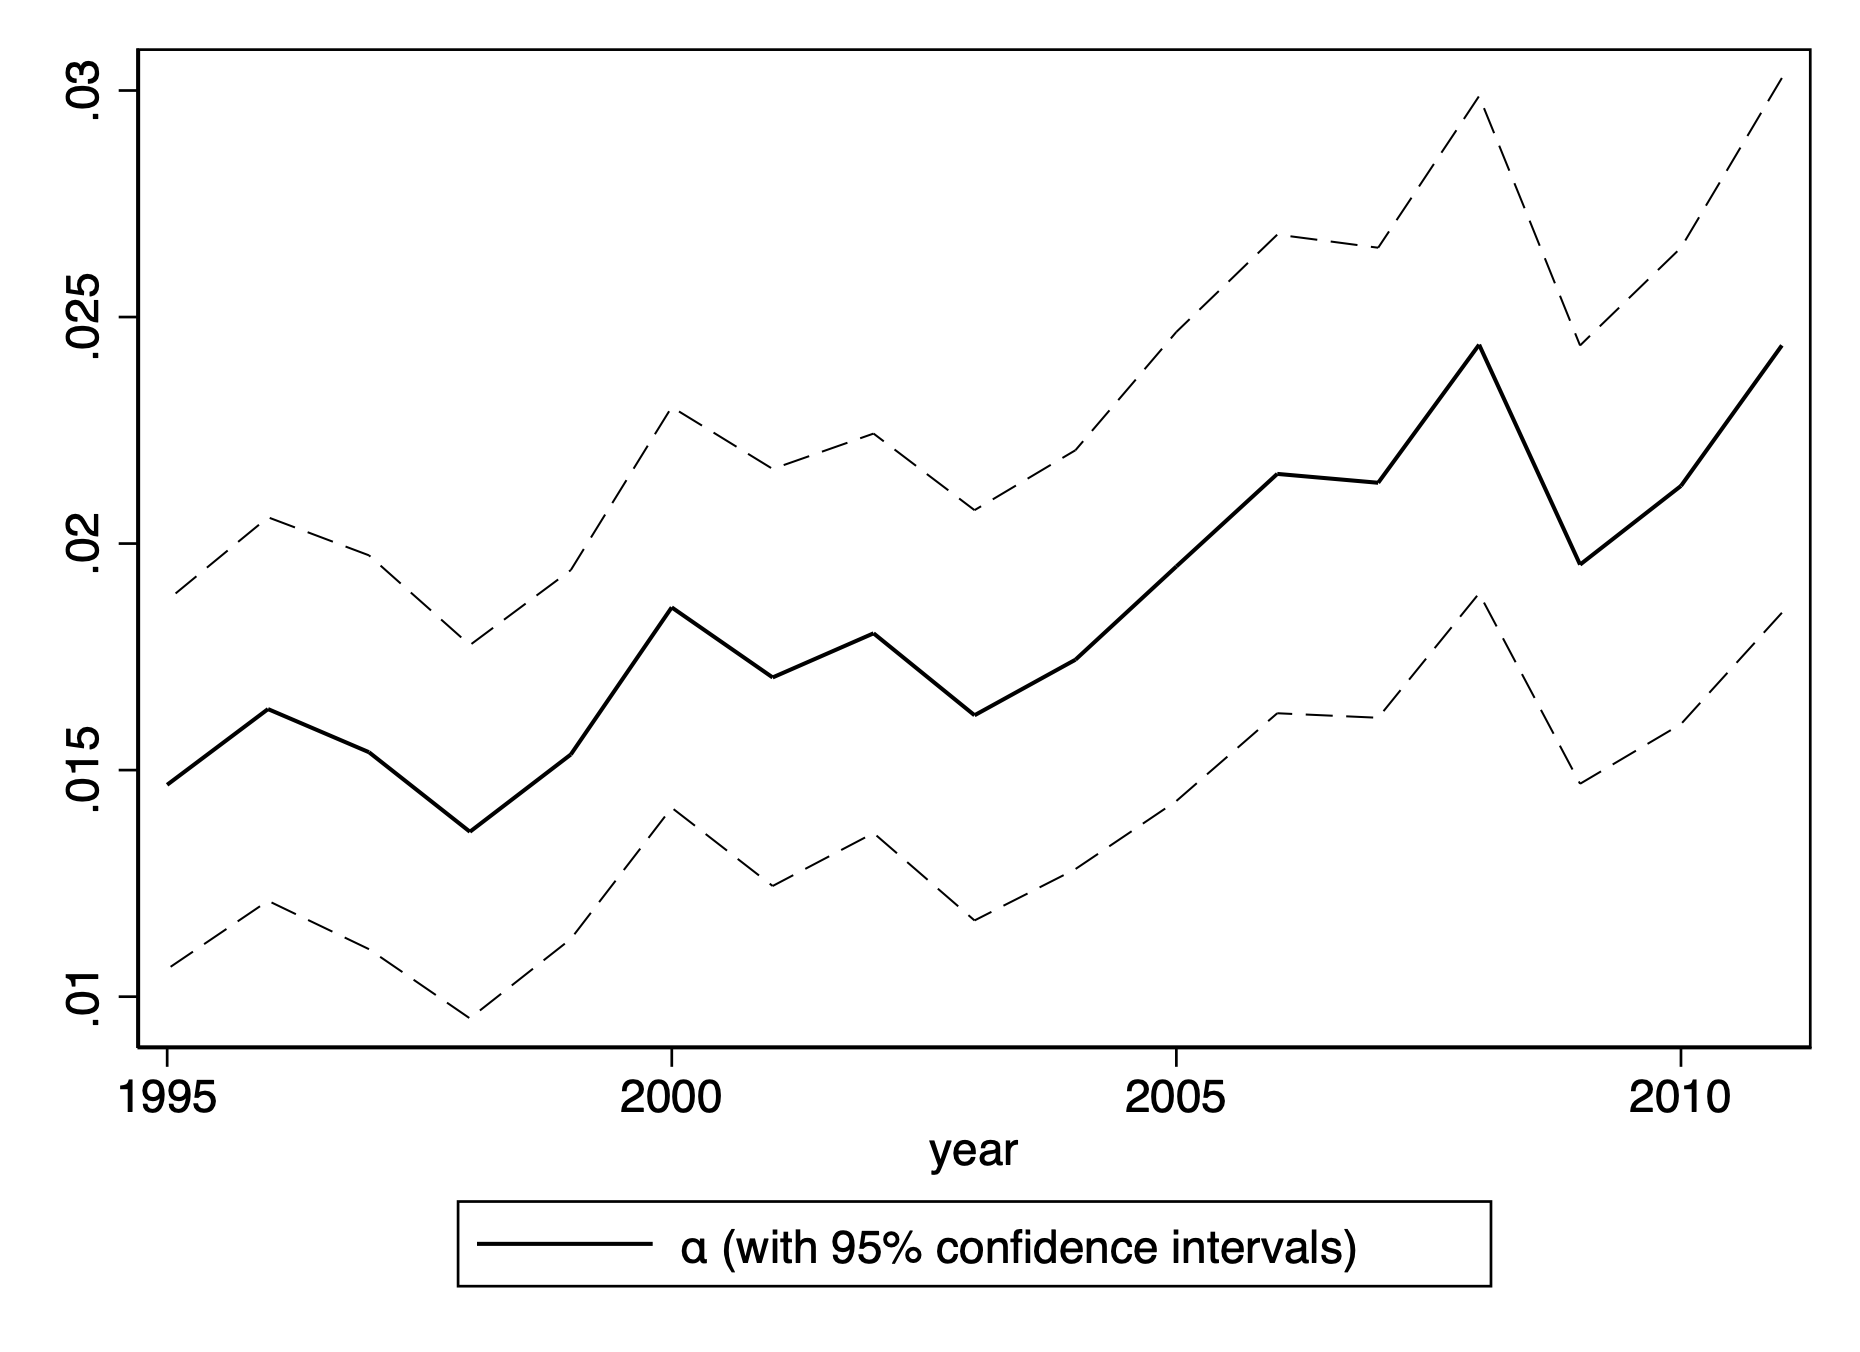
\includegraphics[width=5.0in, height=3.5in]{coef_cst_TIVA_HC}\\
	\end{tabular}
	\label{fig:evolution_cst_TiVA}
	\floatfoot{Sources: TIVA rev3 and authors’ calculations}.
\end{figure}

\begin{figure}[H]
	\centering
	\caption{\footnotesize{\textbf{Comparison between $\overline{s}_{i}^{i,HC}$ and $E1.HC^{i,imp}+E2.HC^{i,dom}$ (TIVA rev. 4)}}}
	\begin{tabular}{c}
		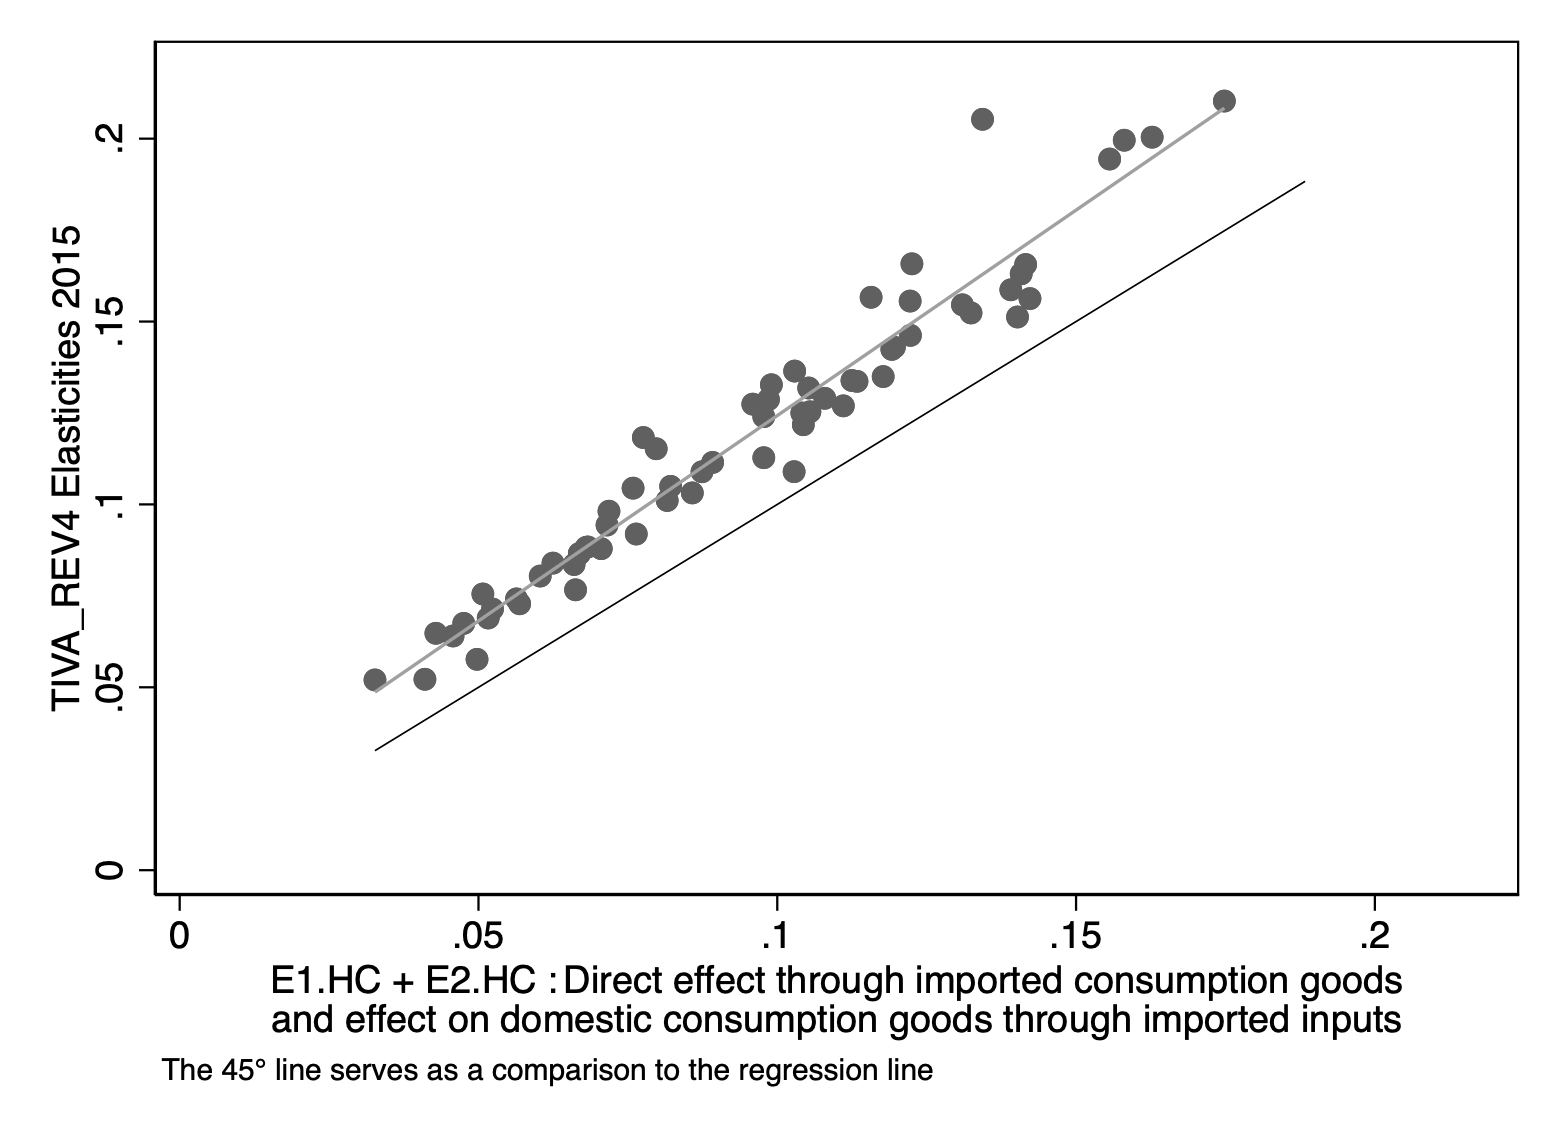
\includegraphics[width=5.0in, height=3.5in]{Comp_s_E1HCE2HC_2015_TIVA_REV4_HC.png}\\
	\end{tabular}
	\label{fig:ratiodir_TiVA_REV4}
	\floatfoot{Sources: TIVA rev4 and authors’ calculations}.
\end{figure}

\begin{figure}[H]
	\centering
	\caption{\footnotesize{\textbf{Evolution of $\beta$ and $R2$ (TIVA rev. 4)}}}
	\begin{tabular}{c}
		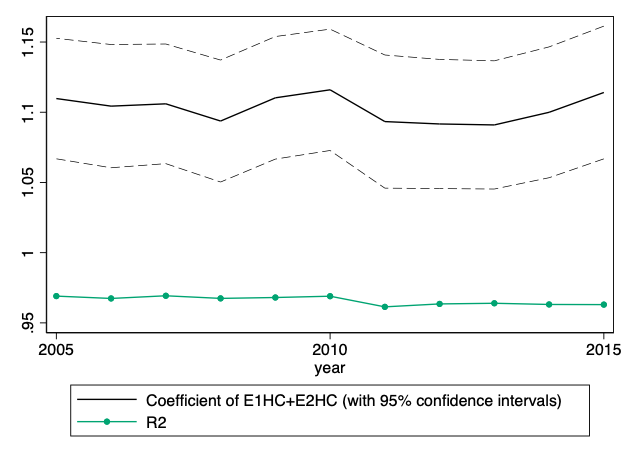
\includegraphics[width=5.0in, height=3.5in]{coef_E_TIVA_REV4_HC}\\
	\end{tabular}
	\label{fig:evolution_b_TiVA_REV4}
	\floatfoot{Sources: TIVA rev4 and authors’ calculations}.
\end{figure}

\begin{figure}[H]
	\centering
	\caption{\footnotesize{\textbf{Time evolution of $\alpha$ (TIVA rev. 4)}}}
	\begin{tabular}{c}
		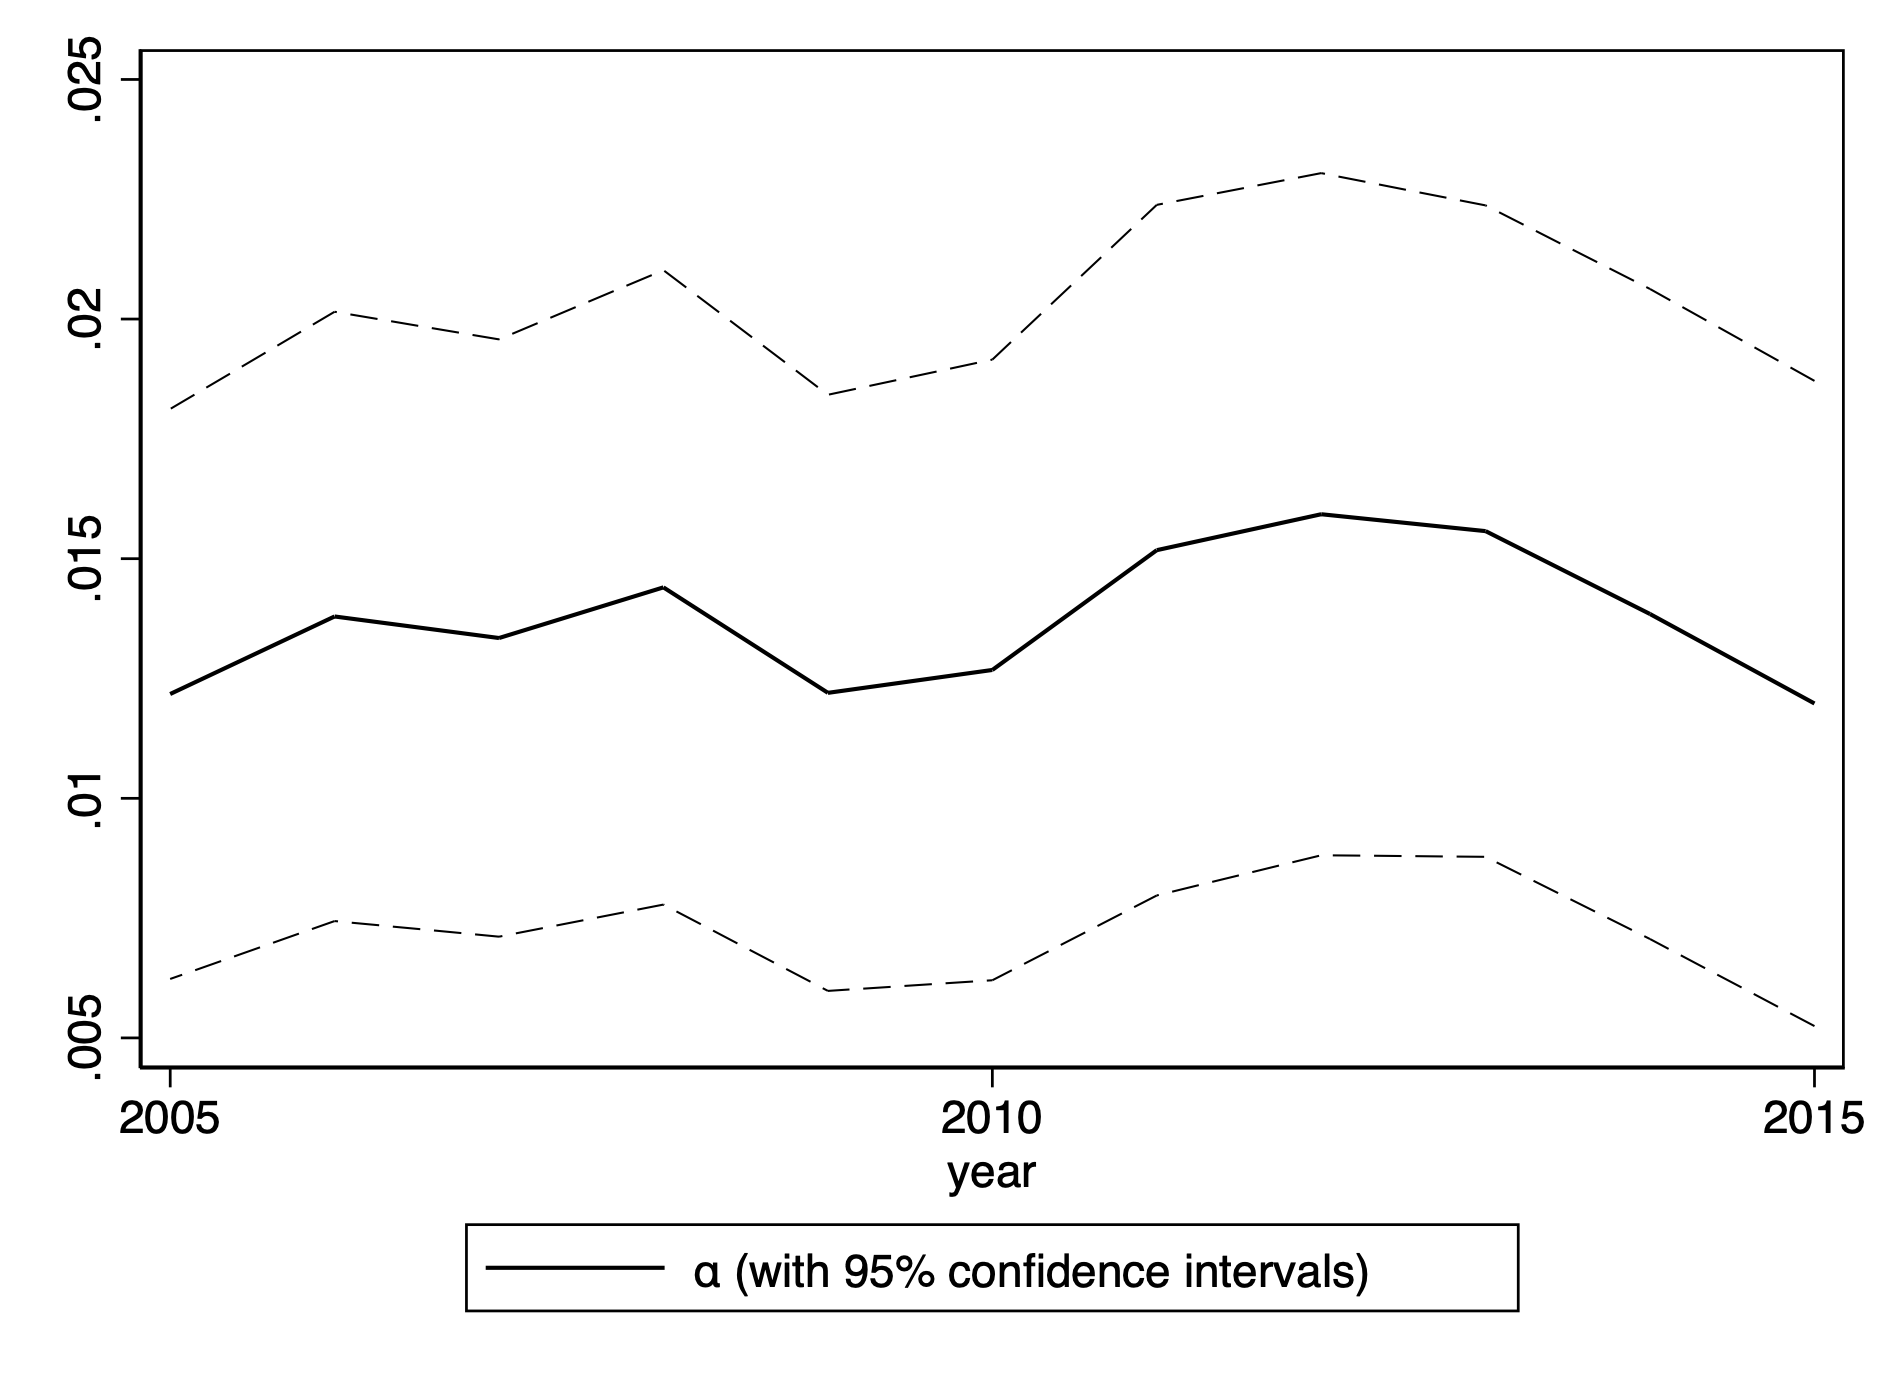
\includegraphics[width=5.0in, height=3.5in]{coef_cst_TIVA_REV4_HC}\\
	\end{tabular}
	\label{fig:evolution_cst_TiVA_REV4}
	\floatfoot{Sources: TIVA rev4 and authors’ calculations}.
\end{figure}


\newpage
\section*{Online Appendix D: Study of the decomposition of the shock in the two-country, one-sector case}\label{AnalyticalAppendix}
\subsection*{The issue}

As a reminder from the paper, where $\overline{s}_{i}^{i,HC}$ is the effect of an exchange rate shock on consumption prices :  
\begin{equation}
\begin{array}{lccl}
\overline{s}_{i}^{i,HC}&=S^i.HC^i=E1.HC^i+E2.HC^i+E3.HC^i+E4.HC^i \\
&=E1.HC^{i,imp}+E2.HC^{i,dom}+E3.HC^{i,imp}+E4.HC^i
\end{array} 
\end{equation}

and

\begin{equation}
\begin{array}{lccl}
S^ i&=&C^i	&+ \left(\hat{C}^i_\$.{\cal B}^i+{C^i}{\tilde{{\cal B}^i}}\right)*{{(I-{\cal A})}^{-1}} \\
S^i &=&\underbrace{C^i}_{\substack{\text{(E1) direct effect through} \\ \text{ imported consumption goods}}}&+ \underbrace{{C^i}{\tilde{{\cal B}^i}}}_{\substack{\text{(E2) effect on} \\ \text{ \emph{domestic} consumption goods} \\ \text{ through \emph{imported} inputs}}}  + \underbrace{\hat{C}^i_\$.{\cal B}^i}_{\substack{\text{(E3)  effect on} \\ \text{\emph{imported} consumption goods} \\ \text{through \emph{domestic} inputs}}} \\ &&+\underbrace {\left( \hat{C}^i_\$.{\cal B}^i + {C^i}{\tilde{{\cal B}^i}}\right)*{{(I-{\cal A})}^{-1}}*{\cal A}}_{\text{(E4) residual}} \\
\end{array}
\end{equation}



When the shock corresponds to an appreciation of the domestic currency, $E1$ and $E2$ reduce country $i$'s consumer prices whereas $E3$ increases them. $E1$ and $E2$ are easy to compute with national input-output matrices, whereas world input-output matrices are needed for computing $E3$ and $E4$.

Unexpectedly, $E3 + E4$ seems to be constant, regardless of the openness rate of the economy (see Figure \ref{fig:ratiodir_WIOD}).


Let us focus on the two-country, one-sector economy : 

\begin{gather*}
E1=C=\left(0,-c\right)
\\
E2=C.\tilde{\cal B}^i=\left(0,-c\right).\left(\begin{matrix}0&0\\a_{2,1}&0\end{matrix}\right)=\left(-c.a_{2,1},0\right)
\\
E3=(c,0).\left(\begin{matrix}0&a_{1,2}\\0&0\end{matrix}\right)=\left(0,c.a_{1,2}\right)
\end{gather*}

\begin{gather*}
E1.HC = \left(0,-c\right).\left(\begin{matrix}1-f\\f\end{matrix}\right)=-f.c
\\
E2.HC=\left(-c.a_{2,1},0\right).\left(\begin{matrix}1-f\\f\end{matrix}\right)=-c.a_{2,1}.\left(1-f\right)
\\ 
E3.HC=\left(0,c.a_{1,2}\right).\left(\begin{matrix}1-f\\f\end{matrix}\right)=f.c.a_{1,2}
\end{gather*}

We do not lose any generality by normalising the shock $c$ to 1. 

And, developped from SAGE :
\begin{gather}
\bar{s}-E1.HC-E2.HC=\left(\begin{array}{r}
-\frac{a_{12} a_{21}^{2} - a_{11} a_{21} a_{22} + {\left(a_{11} - a_{12}\right)} a_{21} - {\left(a_{12} a_{21}^{2} - a_{11} a_{21} a_{22} - {\left(a_{11} - 1\right)} a_{12} + {\left(a_{11} - 2 \, a_{12}\right)} a_{21}\right)} f}{a_{12} a_{21} - {\left(a_{11} - 1\right)} a_{22} + a_{11} - 1}
\end{array}\right)
\end{gather}
We assume that:
$\frac{a_{1,1}}{a_{2,1}}=\frac{1-f}{f}$ and $a_{1,1}+a_{2,1}=a$. \\ 
So
$a_{1,1}=(1-f)a$ and $a_{2,1}=fa$. \\

Then:

\begin{gather}
\bar{s}-E1.HC-E2.HC=\left(\begin{array}{r}
-\frac{{\left(a^{2} a_{12} + a^{2} a_{22} - a^{2}\right)} f^{3} - {\left(2 \, a^{2} a_{22} - 2 \, a^{2} + {\left(a^{2} + a\right)} a_{12}\right)} f^{2} + {\left(a^{2} a_{22} - a^{2} + a_{12}\right)} f}{{\left(a - 1\right)} a_{22} - {\left(a a_{12} + a a_{22} - a\right)} f - a + 1}
\end{array}\right)
\end{gather}

According to SAGE, the derivative of this according to f is: 
\begin{gather*}
\left(\begin{array}{r}
-\frac{{\left({\left(a^{2} a_{12} + a^{2} a_{22} - a^{2}\right)} f^{3} - {\left(2 \, a^{2} a_{22} - 2 \, a^{2} + {\left(a^{2} + a\right)} a_{12}\right)} f^{2} + {\left(a^{2} a_{22} - a^{2} + a_{12}\right)} f\right)} {\left(a a_{12} + a a_{22} - a\right)}}{{\left({\left(a - 1\right)} a_{22} - {\left(a a_{12} + a a_{22} - a\right)} f - a + 1\right)}^{2}} \\
- \frac{a^{2} a_{22} + 3 \, {\left(a^{2} a_{12} + a^{2} a_{22} - a^{2}\right)} f^{2} - a^{2} - 2 \, {\left(2 \, a^{2} a_{22} - 2 \, a^{2} + {\left(a^{2} + a\right)} a_{12}\right)} f + a_{12}}{{\left(a - 1\right)} a_{22} - {\left(a a_{12} + a a_{22} - a\right)} f - a + 1}
\end{array}\right)
\end{gather*}

The sign of this expression is difficult to study. We hence move to a numerical application.

\subsection*{Numerical application}
Based on WIOD 2014, we compute the ratio between value added and production. The computation with the WIOD data is : 
egen total=rowtotal(vAUS1-vROW) and then (161-74)/161=0.54.

To simplify, we assume that the ratio is equal to 0.5.
\begin{gather*}
a_{1,1}+a_{1,2}=a_{2,1}+a_{2,2}=0.5 \\
\frac{a_{1,2}}{a_{1,1}+a_{1,2}}=f \\
a_{2,1}=0.48 \\
a_{2,2}=0.02
\end{gather*}
In that case:

\begin{gather*}
\begin{array}{r}
\bar{s}-E1.HC-E2.HC = \frac{-0.125 \, f^{3} + 0.245 \, f^{2} - 0.11 \, f}{-0.25 \, f - 0.26
}
\end{array}
\end{gather*}

Which yields Figures \ref{fig:resid} and \ref{fig:tous_les_E}.
\begin{figure}[H]
	\begin{center}
		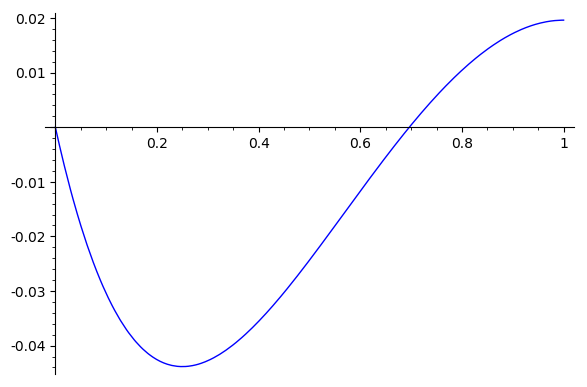
\includegraphics{etude_residu.png}
		\caption{$\bar{s}-E1.HC-E2.HC$ as a function of the openness rate}
		\label{fig:resid}
	\end{center}
\end{figure}

Actual openness rates in the sample vary between 0.15 and 0.5. In that zone, the relationship between the openness rate and the residual is not monotonous (see Figure \ref{fig:resid}).

Figure \ref{fig:tous_les_E} confirms that, in that numerical exercise, the total effect is dominated by the direct effect through imported consumption goods and, to a lesser extent, the effect on domestic consumption goods through imported inputs. 
The other effects are approximately additive if the openness rate is betweem 0.15 and 0.5.

\begin{figure}[H]
	\begin{center}
		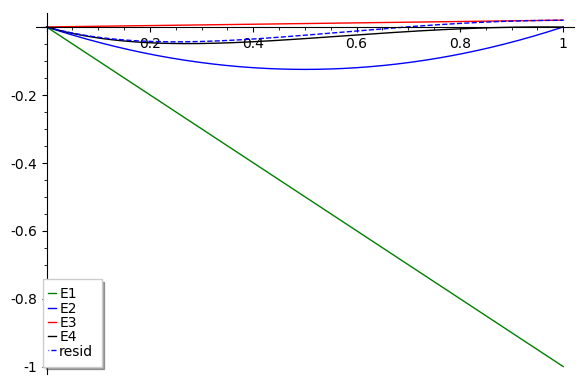
\includegraphics{etude_tous_les_E.png}
		\caption{E1.HC, E2.HC, E3.HC, E4.HC and the "residual"  ($\bar{s}-E1.HC-E2.HC$) as a function of the openness rate}
		\label{fig:tous_les_E}
	\end{center}
\end{figure}

\end{document}
